\section{Experiments}
\label{sec:experiments}

\newcommand{\MethodOne}{\shortstack[c]{Before RLVR}}
\newcommand{\MethodTwo}{\shortstack[c]{RLVR w/o Multi-Hop}}
\newcommand{\MethodThree}{\shortstack[c]{RLVR w/ Multi-Hop}}
\newcolumntype{Y}{>{\centering\arraybackslash}X}
\newlength{\BenchmarkColWidth}
\newlength{\ResultColWidth}
\setlength{\BenchmarkColWidth}{0.18\linewidth}
\setlength{\ResultColWidth}{\dimexpr(\linewidth-\BenchmarkColWidth)/3\relax}
\newcommand{\ExperimentHeaderRow}{%
\multicolumn{4}{@{}l@{}}{%
  \begingroup
  \setlength{\fboxsep}{0pt}%
  \colorbox{black!5}{%
    \parbox{\linewidth}{%
      \strut
      \makebox[\BenchmarkColWidth][l]{Benchmark}%
      \makebox[\ResultColWidth][c]{\MethodOne}%
      \makebox[\ResultColWidth][c]{\MethodTwo}%
      \makebox[\ResultColWidth][c]{\MethodThree}%
      \strut
    }%
  }%
  \endgroup
}%
\\}


We evaluate HopChain from three complementary angles.
First, we test whether adding multi-hop data to RLVR training based on the original RLVR data improves general vision-language reasoning across model scales and benchmark families (\cref{sec:exp-main-results}).
Second, we examine whether the full multi-hop formulation is necessary, rather than weaker single-hop or truncated-hop variants (\cref{sec:exp-hop-structure-ablation}).
Third, we analyze whether the observed gains align with our central claims about long-CoT robustness, data difficulty coverage, and broad correction of diverse failure modes (\cref{sec:exp-analysis}).

\subsection{Experimental Setup}
We evaluate two models, \textbf{Qwen3.5-35B-A3B} and \textbf{Qwen3.5-397B-A17B}~\CiteParen{qwen35blog}, under three settings: \texttt{Before RLVR}, \texttt{RLVR w/o Multi-Hop}, and \texttt{RLVR w/ Multi-Hop}.
Here, \texttt{Before RLVR} denotes the model after SFT and before RLVR, which serves as the shared starting point for both RLVR settings; \texttt{RLVR w/o Multi-Hop} denotes RLVR training on the original RLVR data only, while \texttt{RLVR w/ Multi-Hop} denotes RLVR training on a mixture of the original RLVR data and our synthesized multi-hop data.
Unless otherwise stated, the SFT data and the original RLVR data used in these experiments are pre-final internal versions, rather than the final official Qwen3.5 data recipe.
For Qwen3.5-35B-A3B, each rollout samples 16 responses for each of 256 queries, uses a mini-batch size of 64 queries, and runs for 1000 gradient steps.
Qwen3.5-397B-A17B follows the same rollout configuration in general, except that the mini-batch size is increased to 128 queries and the total number of gradient steps is 800.
For both models, RLVR training uses the SAPO algorithm with a learning rate of $2.0 \times 10^{-6}$, while other hyperparameters follow the original SAPO paper~\CiteParen{sapo}.




\begin{table}[t]
\centering
\caption{Results of Qwen3.5-35B-A3B. \texttt{Before RLVR} denotes the model after SFT but before RLVR. \texttt{RLVR w/o Multi-Hop} denotes RLVR training on the original RLVR data only. \texttt{RLVR w/ Multi-Hop} denotes RLVR training on the original RLVR data plus the multi-hop data synthesized by HopChain.}
\vspace{-5pt}
\label{tab:exp-35b}
{\renewcommand{\arraystretch}{1.10}
\begin{tabularx}{\linewidth}{@{}>{\raggedright\arraybackslash}p{0.18\linewidth}YYY@{}}
\toprule
\ExperimentHeaderRow
\midrule
\rowcolor{black!3}
\multicolumn{4}{l}{\textbf{STEM and Puzzle}} \\
MathVision & 61.97 & 73.71 & \best{76.05} \\
MMMU Pro & 66.07 & 69.25 & \best{70.64} \\
MMMU & 75.89 & \best{78.89} & 78.33 \\
Mathvista(mini) & 82.80 & \best{85.50} & 85.00 \\
BabyVision & 14.95 & 21.91 & \best{22.68} \\
ZEROBench & 1 & 1 & \best{3} \\
EMMA(mini) & 41.88 & 53.00 & \best{58.00} \\
LogicVista & 63.85 & 74.66 & \best{75.56} \\
\midrule
\rowcolor{black!3}
\multicolumn{4}{l}{\textbf{General VQA}} \\
MMBench$_{\scriptscriptstyle\text{CN-DEV-V1.1}}$ & 87.46 & 90.17 & \best{90.48} \\
MMBench$_{\scriptscriptstyle\text{EN-DEV-V1.1}}$ & 88.47 & 90.63 & \best{91.49} \\
RealWorldQA & 75.42 & 78.17 & \best{79.35} \\
MMStar & 75.20 & 78.53 & \best{78.60} \\
HallusionBench & 66.49 & \best{66.64} & 66.50 \\
AI2D\_TEST & 88.44 & 90.87 & \best{91.29} \\
ERQA & 44.50 & 48.25 & \best{51.38} \\
\midrule
\rowcolor{black!3}
\multicolumn{4}{l}{\textbf{Text Recognition and Document Understanding}} \\
CharXiv & 61.30 & 69.00 & \best{73.10} \\
DocVQA\_VAL & 95.00 & 95.13 & \best{95.55} \\
InfoVQA\_VAL & 86.81 & 87.44 & \best{90.17} \\
\midrule
\rowcolor{black!3}
\multicolumn{4}{l}{\textbf{Video Understanding}} \\
VideoMME$_{\text{w/o sub.}}$ & 73.41 & 74.63 & \best{75.00} \\
VideoMMMU & 70.67 & 73.33 & \best{74.78} \\
MMVUCOT & 63.70 & 65.80 & \best{68.90} \\
MVBench & 69.18 & 69.95 & \best{70.73} \\
LVBench & 51.13 & \best{54.49} & 53.20 \\
MLVU (M-Avg) & 77.92 & 77.69 & \best{79.53} \\
\bottomrule
\end{tabularx}}
\end{table}

\begin{table}[t]
\centering
\caption{Results of Qwen3.5-397B-A17B, the larger model counterpart of \cref{tab:exp-35b}. \texttt{Before RLVR} denotes the model after SFT but before RLVR. \texttt{RLVR w/o Multi-Hop} denotes RLVR training on the original RLVR data only. \texttt{RLVR w/ Multi-Hop} denotes RLVR training on the original RLVR data plus the multi-hop data synthesized by HopChain.}
\vspace{-5pt}
\label{tab:exp-397b}
{\renewcommand{\arraystretch}{1.10}
\begin{tabularx}{\linewidth}{@{}>{\raggedright\arraybackslash}p{0.18\linewidth}YYY@{}}
\toprule
\ExperimentHeaderRow
\midrule
\rowcolor{black!3}
\multicolumn{4}{l}{\textbf{STEM and Puzzle}} \\
MathVision & 77.38 & 81.68 & \best{83.71} \\
MMMU Pro & 73.03 & 75.06 & \best{76.47} \\
MMMU & 79.78 & 81.67 & \best{82.89} \\
Mathvista(mini) & 87.50 & 88.30 & \best{89.00} \\
BabyVision & 17.01 & 28.61 & \best{32.22} \\
ZEROBench & 3 & 4 & \best{8} \\
EMMA(mini) & 58.13 & 66.25 & \best{69.00} \\
LogicVista & 75.62 & 80.69 & \best{81.59} \\
\midrule
\rowcolor{black!3}
\multicolumn{4}{l}{\textbf{General VQA}} \\
MMBench$_{\scriptscriptstyle\text{CN-DEV-V1.1}}$ & 89.47 & 91.41 & \best{91.72} \\
MMBench$_{\scriptscriptstyle\text{EN-DEV-V1.1}}$ & 90.71 & \best{92.49} & 91.56 \\
RealWorldQA & 79.87 & 79.87 & \best{81.70} \\
MMStar & 80.00 & \best{81.73} & 80.67 \\
HallusionBench & 65.76 & 67.48 & \best{67.86} \\
AI2D\_TEST & 91.45 & 92.81 & \best{92.97} \\
ERQA & 53.75 & \best{60.50} & 60.00 \\
\midrule
\rowcolor{black!3}
\multicolumn{4}{l}{\textbf{Text Recognition and Document Understanding}} \\
CharXiv & 70.00 & 74.60 & \best{77.20} \\
DocVQA\_VAL & 95.93 & 95.98 & \best{96.03} \\
InfoVQA\_VAL & 90.42 & 90.83 & \best{92.20} \\
\midrule
\rowcolor{black!3}
\multicolumn{4}{l}{\textbf{Video Understanding}} \\
VideoMME$_{\text{w/o sub.}}$ & 76.56 & 78.30 & \best{80.41} \\
VideoMMMU & 76.67 & 78.89 & \best{80.00} \\
MMVUCOT & 70.20 & 72.30 & \best{72.50} \\
MVBench & 69.63 & 73.03 & \best{73.31} \\
LVBench & 58.30 & \best{59.13} & 59.07 \\
MLVU (M-Avg) & 81.46 & 82.43 & \best{82.52} \\
\bottomrule
\end{tabularx}}
\end{table}

\paragraph{Image Filtering.}
Before multi-hop query synthesis, we filter images to retain cases that are genuinely useful for long vision-language reasoning.
The selection prompt in Appendix~\ref{app:image-select-prompt} is designed to favor images that are perceptually challenging for standard vision models, such as those involving occlusion, dense but still analyzable objects, unusual poses, complex interactions, fine-grained distinctions, or difficult lighting, while filtering out images that are too low-quality or too annotation-impractical to support verifiable reasoning.
To balance quality and throughput, we use a two-stage pipeline.
We first apply Qwen3-VL-235B-A22B-Thinking to a small subset of images with the image-selection prompt and keep the accepted images as the initial set of selected images.
We then use this initial set of selected images together with the large model's outputs to perform supervised fine-tuning (SFT) on a smaller model, Qwen3-VL-30B-A3B-Thinking, specialized for image filtering.
Next, we run this smaller model over all remaining images to obtain a coarse screening result.
Finally, we send the images retained by the coarse screening back to Qwen3-VL-235B-A22B-Thinking for a second, finer filtering pass, yielding a second set of selected images.
The union of the initial set of selected images and the second set of selected images forms the final pool of images used for multi-hop data construction.
Based on the filtered image pool above, we construct multi-hop queries with HopChain and then filter out overly easy samples using a weaker model and the pre-RLVR model, yielding about $6k$--$8k$ multi-hop RLVR samples for each model.
In addition, we use a similar amount of math RLVR data as the original RLVR data.

\paragraph{Benchmarks.}
We evaluate 24 benchmarks across 4 categories.
For \textbf{STEM and puzzle} reasoning, we use MathVision~\CiteParen{wang2024mathvision}, MMMU-Pro~\CiteParen{yue2025mmmupro}, MMMU~\CiteParen{yue2024mmmu}, MathVista~\CiteParen{lu2024mathvista}, BabyVision~\CiteParen{chen2026babyvision}, ZeroBench~\CiteParen{roberts2025zerobench}, EMMA~\CiteParen{hao2025emma}, and LogicVista~\CiteParen{xiao2024logicvista}.
For \textbf{general VQA}, we use MMBench~\CiteParen{liu2023mmbench}, RealWorldQA~\CiteParen{xai2024realworldqa}, MMStar~\CiteParen{chen2024mmstar}, HallusionBench~\CiteParen{guan2024hallusionbench}, AI2D~\CiteParen{kembhavi2016diagram}, and ERQA~\CiteParen{deepmind2025erqa}.
For \textbf{text recognition and document understanding}, we use CharXiv~\CiteParen{wang2024charxiv}, DocVQA~\CiteParen{mathew2021docvqa}, and InfographicVQA (reported as \texttt{InfoVQA\_VAL})~\CiteParen{mathew2021infographicvqa}.
For \textbf{video understanding}, we use Video-MME~\CiteParen{fu2025videomme}, Video-MMMU~\CiteParen{hu2025videommmu}, MVBench~\CiteParen{li2024mvbench}, LVBench~\CiteParen{wang2024lvbench}, MLVU~\CiteParen{zhou2024mlvu}, and MMVU (reported as \texttt{MMVUCOT})~\CiteParen{zhao2025mmvu}.

\subsection{Main Benchmark Results}
\label{sec:exp-main-results}
Tables~\ref{tab:exp-35b} and~\ref{tab:exp-397b} report the main benchmark results on Qwen3.5-35B-A3B and Qwen3.5-397B-A17B, respectively.
RLVR on the original RLVR data (i.e., \texttt{RLVR w/o Multi-Hop}) already improves the \texttt{Before RLVR} models on many benchmarks, but augmenting the original RLVR data with the multi-hop data synthesized by HopChain (i.e., \texttt{RLVR w/ Multi-Hop}) yields further gains on the majority of benchmarks for both model scales.
These gains are broad rather than isolated.
Importantly, our multi-hop data is not synthesized to target any specific benchmark. Even so, it delivers broad gains on the majority of benchmarks, suggesting that HopChain improves generalizable vision-language reasoning rather than overfitting to benchmark-specific patterns.
Quantitatively, \texttt{RLVR w/ Multi-Hop} improves 20 out of 24 benchmarks for both Qwen3.5-35B-A3B and Qwen3.5-397B-A17B.
For Qwen3.5-35B-A3B, the gains cover 6/8 STEM-and-puzzle benchmarks (MathVision, MMMU-Pro, BabyVision, ZeroBench, EMMA, and LogicVista), 6/7 general-VQA benchmarks (MMBench-CN, MMBench-EN, RealWorldQA, MMStar, AI2D, and ERQA), all 3 text-and-document benchmarks (CharXiv, DocVQA, and InfoVQA), and 5/6 video benchmarks (Video-MME, VideoMMMU, MMVUCOT, MVBench, and MLVU).
For Qwen3.5-397B-A17B, the gains are similarly broad: all 8 STEM-and-puzzle benchmarks improve (MathVision, MMMU-Pro, MMMU, MathVista, BabyVision, ZeroBench, EMMA, and LogicVista), along with 4/7 general-VQA benchmarks (MMBench-CN, RealWorldQA, HallusionBench, and AI2D), all 3 text-and-document benchmarks (CharXiv, DocVQA, and InfoVQA), and 5/6 video benchmarks (Video-MME, VideoMMMU, MMVUCOT, MVBench, and MLVU).
These broad quantitative gains are also reflected qualitatively: \Cref{fig:qualitative_examples} shows representative cases in which adding multi-hop data corrects failures made by \texttt{RLVR w/o Multi-Hop}.
Notably, although our multi-hop data is synthesized from images, the improvement transfers strongly to video understanding: video benchmarks improve on 5 out of 6 tasks for both model scales, indicating substantial cross-domain generalization rather than narrow overfitting to image-only training signals.
Across the two tables, the improvements cover all four benchmark families, with only a small number of regressions, indicating that multi-hop data acts as a composable RLVR training signal rather than a narrow task-specific trick.





\subsection{Ablation on Hop Structure: Single-Hop vs. Half-Multi-Hop vs. Multi-Hop}
\label{sec:exp-hop-structure-ablation}
To test whether preserving complex, long hop chains during training is necessary, we compare three training-query settings on the subset of benchmarks shared by all three runs.
In \texttt{RLVR w/ Single Hop}, each multi-hop training query is reduced to only its final hop; in \texttt{RLVR w/ Half-Multi-Hop}, the first half of the chain is removed and only the latter half is kept; and in \texttt{RLVR w/ Multi-Hop}, the full query is kept.

\newcommand{\MethodSingleHop}{\shortstack[c]{RLVR w/\\Single Hop}}
\newcommand{\MethodHalfHop}{\shortstack[c]{RLVR w/\\Half-Multi-Hop}}
\newcommand{\MethodMultiHop}{\shortstack[c]{RLVR w/\\Multi-Hop}}
\newlength{\HopBenchmarkColWidth}
\newlength{\HopResultColWidth}
\setlength{\HopBenchmarkColWidth}{0.28\linewidth}
\setlength{\HopResultColWidth}{\dimexpr(\linewidth-\HopBenchmarkColWidth)/3\relax}
\newcommand{\HopComparisonHeaderRow}{%
\multicolumn{4}{@{}l@{}}{%
  \begingroup
  \setlength{\fboxsep}{0pt}%
  \colorbox{black!5}{%
    \parbox{\linewidth}{%
      \strut
      \makebox[\HopBenchmarkColWidth][l]{\parbox[c][2.6\baselineskip][c]{\HopBenchmarkColWidth}{\raggedright Benchmark}}%
      \makebox[\HopResultColWidth][c]{\parbox[c][2.6\baselineskip][c]{\HopResultColWidth}{\centering \MethodSingleHop}}%
      \makebox[\HopResultColWidth][c]{\parbox[c][2.6\baselineskip][c]{\HopResultColWidth}{\centering \MethodHalfHop}}%
      \makebox[\HopResultColWidth][c]{\parbox[c][2.6\baselineskip][c]{\HopResultColWidth}{\centering \MethodMultiHop}}%
      \strut
    }%
  }%
  \endgroup
}%
\\}

A benchmark-level comparison on five representative tasks is shown in \cref{fig:table3-representive-benchmarks}.
On MathVision, MMMU Pro, RealWorldQA, ERQA, and VideoMMMU, the ordering is consistent: \texttt{RLVR w/ Multi-Hop} performs best, followed by \texttt{RLVR w/ Half-Multi-Hop}, and then \texttt{RLVR w/ Single Hop}.
This per-benchmark ordering is also reflected in the aggregate: averaged across these five representative benchmarks, the score drops from 70.4 for \texttt{RLVR w/ Multi-Hop} to 66.7 for \texttt{RLVR w/ Half-Multi-Hop} and 64.3 for \texttt{RLVR w/ Single Hop}.
This pattern shows that the benefit does not come from collapsing the training queries to the last hop or to a shortened chain; preserving longer cross-hop dependencies is important.

\begin{figure}[t]
\centering
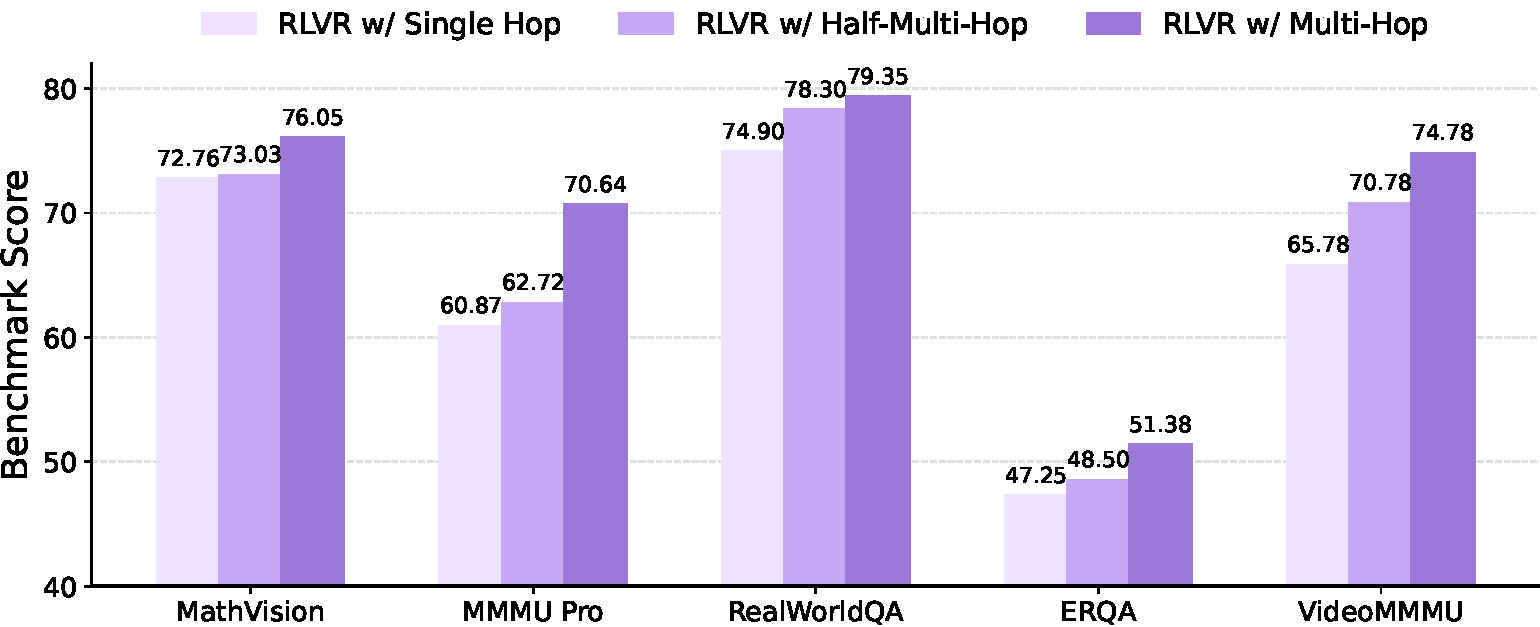
\includegraphics[width=\textwidth]{imgs/table3_representive_benchmarks.pdf}
\caption{Benchmark-level comparison on Qwen3.5-35B-A3B under three training-query settings. \texttt{RLVR w/ Single Hop} simplifies each multi-hop training query to only its final hop, \texttt{RLVR w/ Half-Multi-Hop} removes the first half of the hops and keeps only the latter half, and \texttt{RLVR w/ Multi-Hop} uses the full multi-hop training queries. We evaluate the resulting models on five representative benchmarks, namely MathVision, MMMU Pro, RealWorldQA, ERQA, and VideoMMMU, and plot the benchmark score for each setting. Across all five benchmarks, the full multi-hop setting performs best, showing that preserving the complete multi-hop structure during training is more effective than shortening the query chain.}
\label{fig:table3-representive-benchmarks}
\end{figure}

\subsection{Analysis}
\label{sec:exp-analysis}
\paragraph{Analysis by Reasoning Length.}
If HopChain primarily strengthens long-CoT reasoning, its advantage should persist as response chains become longer.
\Cref{fig:ultra_long_cot_advantage} tests exactly this on Qwen3.5-397B-A17B by binning benchmark responses by response token count.
The advantage of \texttt{RLVR w/ Multi-Hop} over \texttt{RLVR w/o Multi-Hop} remains visible across the bins and is often larger in the ultra-long-response regime.
This supports the interpretation that HopChain improves robust chained reasoning over long outputs, rather than only helping on short or easy responses.

\begin{figure}[t]
\centering
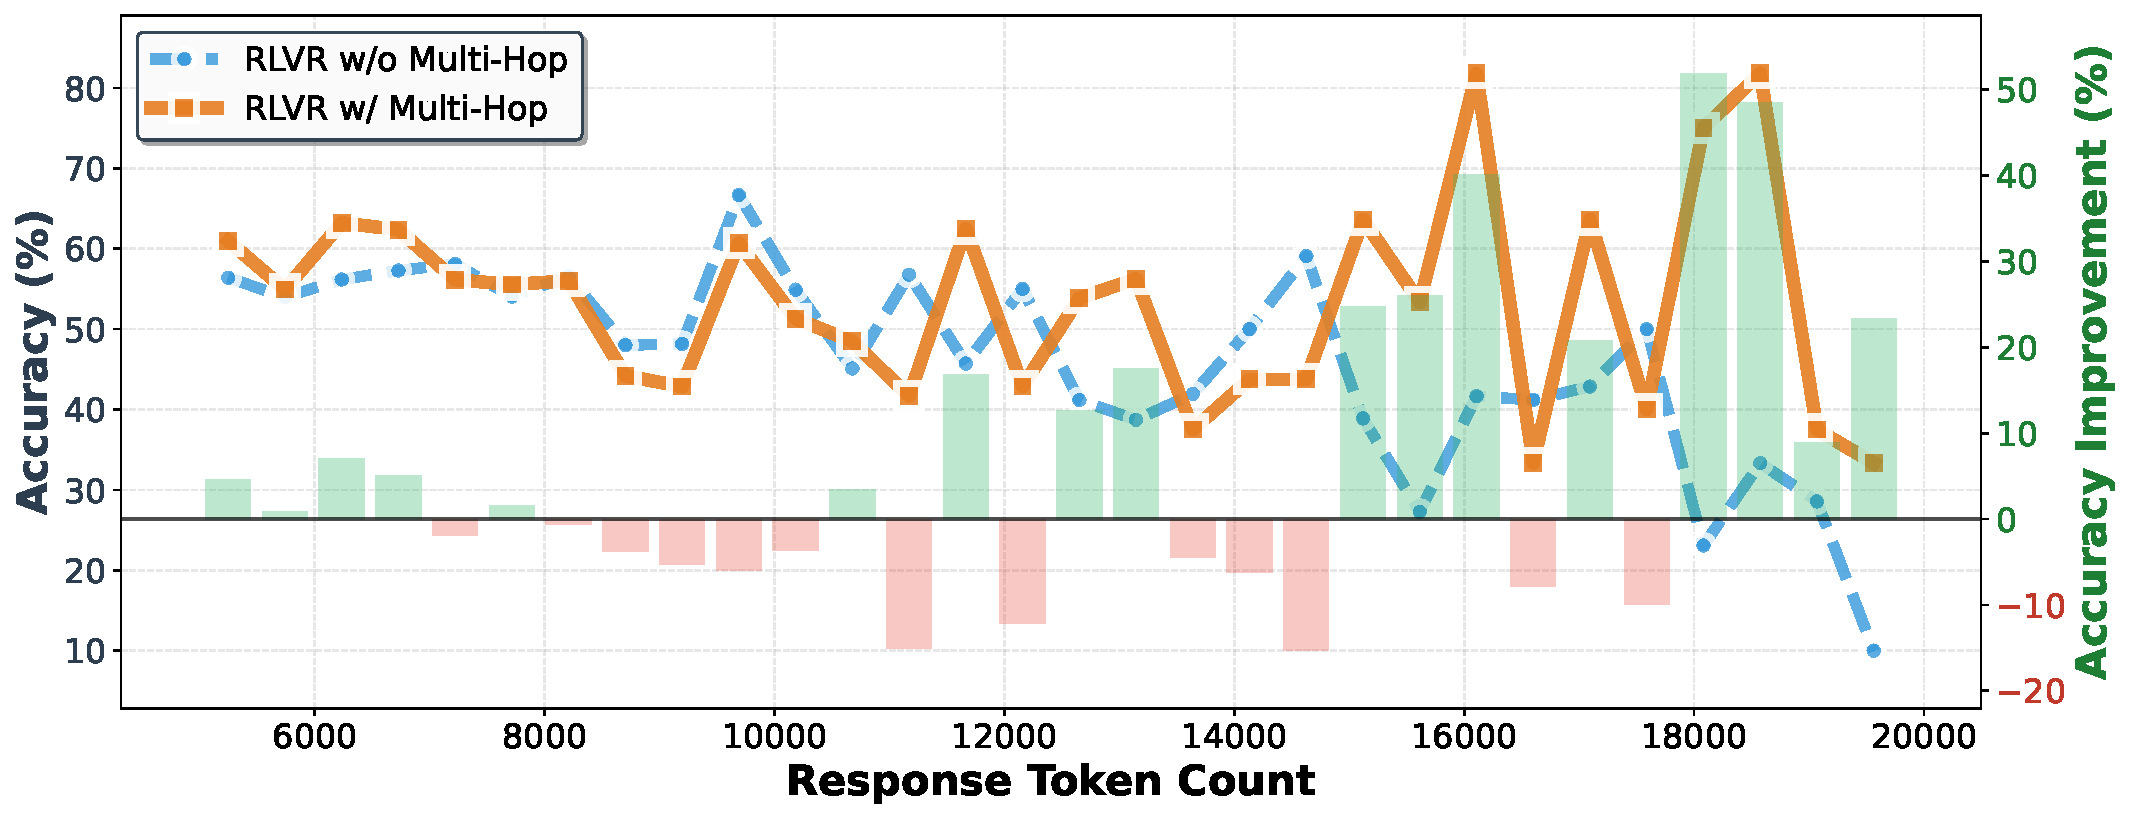
\includegraphics[width=\textwidth]{imgs/ultra_long_cot_advantage.pdf}
\caption{Performance as a function of response length, aggregated from the benchmark evaluation results of Qwen3.5-397B-A17B in \cref{tab:exp-397b}. The blue dashed line and the orange solid line show the accuracies of \texttt{RLVR w/o Multi-Hop} and \texttt{RLVR w/ Multi-Hop}, respectively, across bins of increasing response token count, while the bars show the corresponding accuracy improvement of \texttt{RLVR w/ Multi-Hop} over \texttt{RLVR w/o Multi-Hop} on the right axis. The advantage of multi-hop training remains evident on long responses and is especially pronounced in the ultra-long-CoT region.}
\label{fig:ultra_long_cot_advantage}
\end{figure}

\paragraph{Difficulty Coverage Across Model Scales.}
A useful multi-hop training set should cover a broad range of difficulties, rather than collapsing to queries that are either trivial or essentially unsolvable.
\Cref{fig:turbo_vs_plus_success_rate_histogram} measures this by independently sampling eight responses for each multi-hop query and grouping the query by how many sampled responses are correct.
For both Qwen3.5-35B-A3B and Qwen3.5-397B-A17B, more than half of the queries fall into the \texttt{Partially Correct} regime, and the distribution spans multiple success buckets.
This indicates that the synthesized multi-hop data covers a broad difficulty range and can provide a useful RLVR training signal to models of different sizes and capability levels.

\begin{figure}[t]
\centering
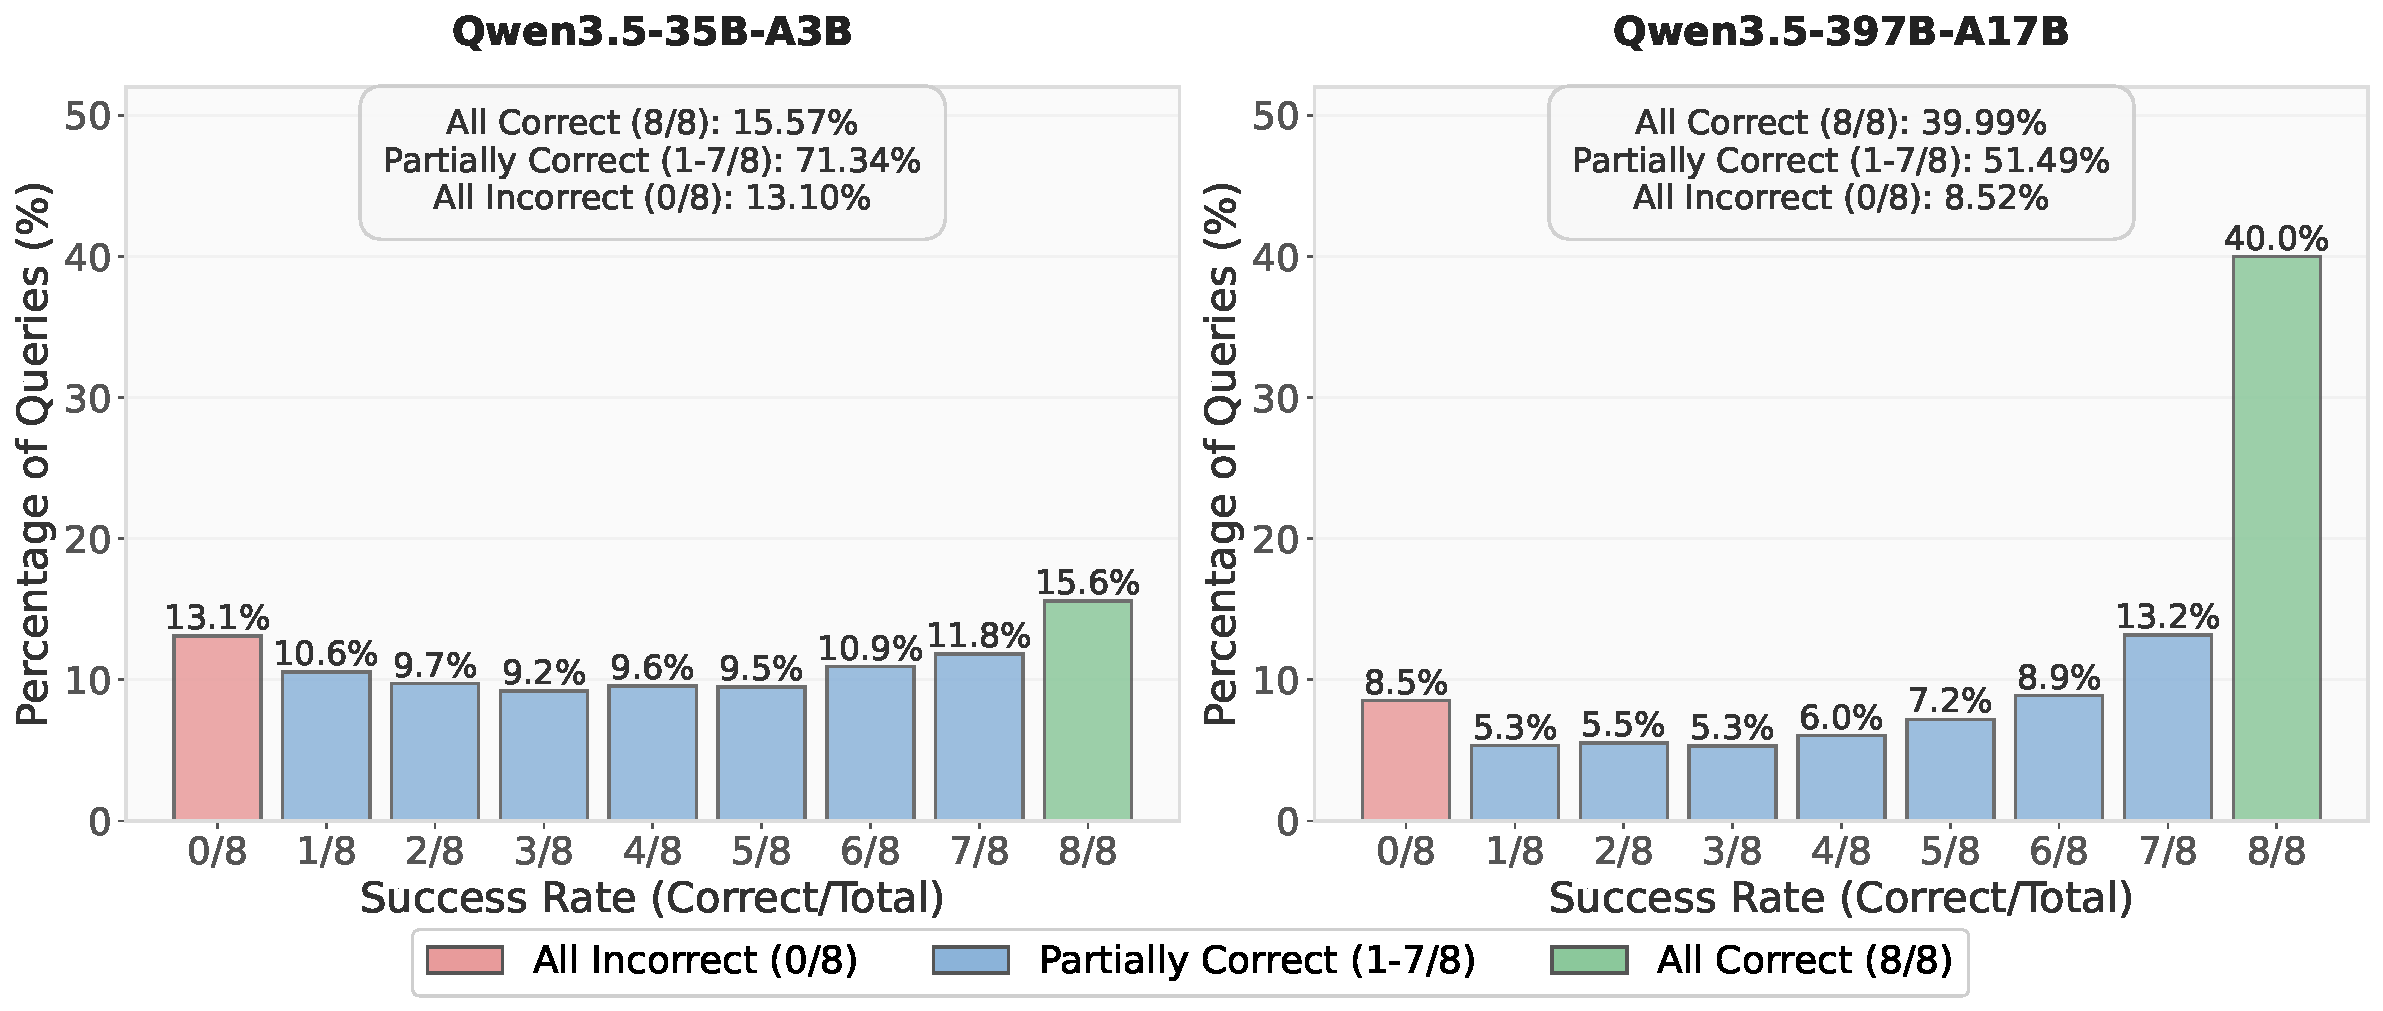
\includegraphics[width=\textwidth]{imgs/turbo_vs_plus_success_rate_histogram.pdf}
\caption{Query-level success-rate distributions for Qwen3.5-35B-A3B and Qwen3.5-397B-A17B. For each multi-hop query, we independently sample eight responses and bucket the query by how many of the eight are correct, from \texttt{0/8} to \texttt{8/8}. For both models, more than half of the queries fall into the \texttt{Partially Correct} regime, and the queries are distributed across multiple success buckets. This suggests that the synthesized multi-hop data spans a broad difficulty range and is suitable for RLVR training across models of different sizes and capability levels.}
\label{fig:turbo_vs_plus_success_rate_histogram}
\end{figure}

\paragraph{Error-Type Analysis.}
Finally, we ask whether multi-hop augmentation fixes only a narrow corner of the error space or yields broader gains.
\Cref{fig:error_distribution} analyzes the original error types of the cases where \texttt{RLVR w/ Multi-Hop} corrects an error made by \texttt{RLVR w/o Multi-Hop}.
Compared with the baseline error profile in \cref{fig:error_distribution}, the corrected-case distribution is broadly similar: perception errors remain the largest group, reasoning errors remain the second largest, and knowledge, hallucination, and other errors are also represented.
The subtype breakdowns in \Cref{fig:improve_error_distribution} further show that these improvements extend across diverse subcategories, covering chart and text misreads, object misidentification, spatial and counting errors, as well as logic, math, temporal, and causal reasoning errors.
Taken together, the close correspondence to the baseline error distribution in \cref{fig:error_distribution} and the broad subtype gains in \cref{fig:improve_error_distribution} suggest that HopChain does not only patch a single narrow failure type; instead, it yields broad gains across the diverse failure modes in long-CoT vision-language reasoning.

\begin{figure}[t]
\centering
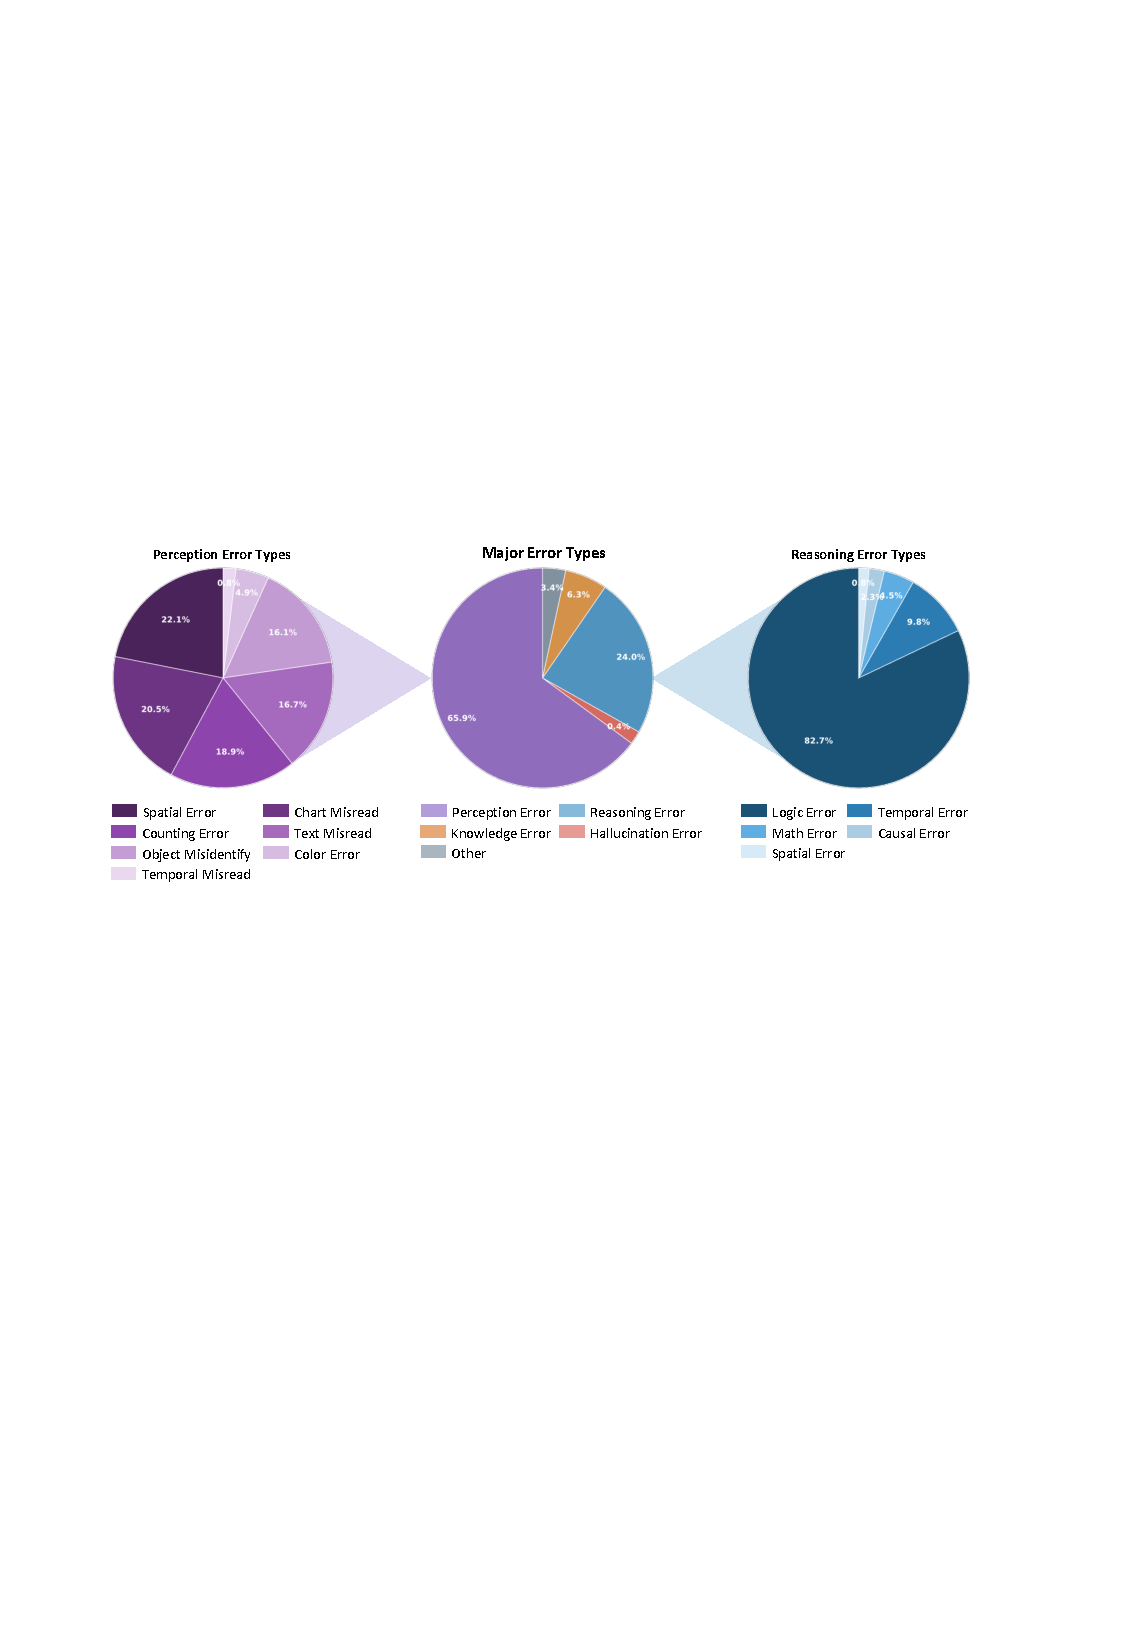
\includegraphics[width=\textwidth]{imgs/improved_categories.pdf}
\caption{Error distribution of the original \texttt{RLVR w/o Multi-Hop} errors among the cases where \texttt{RLVR w/ Multi-Hop} improves over \texttt{RLVR w/o Multi-Hop} on the benchmarks in \cref{tab:exp-35b,tab:exp-397b}. \textbf{Center pie chart:} the major error categories of the corrected cases, indicating which types of baseline errors are most often fixed after adding multi-hop data. \textbf{Left pie chart:} the subtype breakdown of corrected perception errors. \textbf{Right pie chart:} the subtype breakdown of corrected reasoning errors. With \cref{fig:error_distribution}, this figure shows that the multi-hop data synthesized by HopChain can improve models in broad, generalizable domains.}
\label{fig:improve_error_distribution}
\end{figure}
